\begin{figure}
\includegraphics[width=0.6in]{output/1.models/test_watson/watson_1_true.png}\\ 
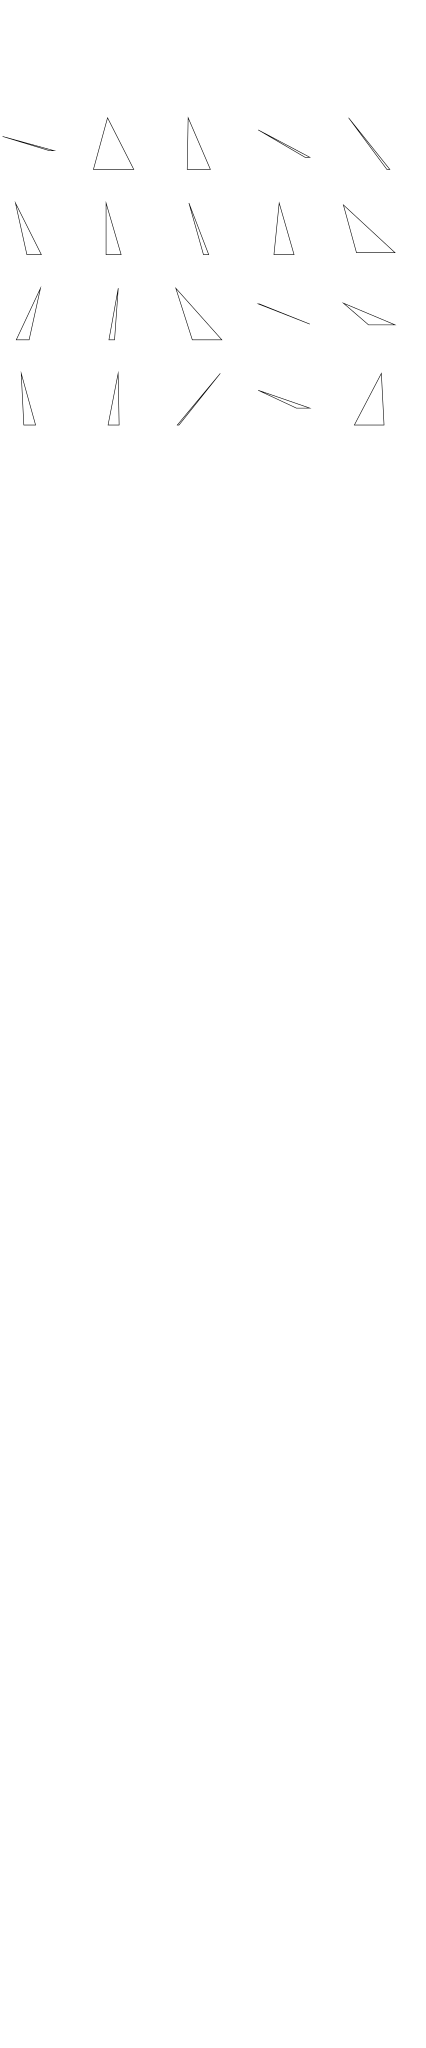
\includegraphics[width=4in]{output/1.models/test_watson/watson_1_samples.png}\\ 
\includegraphics[width=0.6in]{output/1.models/test_watson/watson_1_est.png}
\caption{Experimenting with the Watson distribution, part 1. In the first row, the original triangle $T$. Subsequent rows are samples from Watson$(T,30.00)$. The final row is the mode of the estimated Watson distribution. The estimated concentration was $25.59$.}
\label{fig-watson-1}
\end{figure}

\begin{figure}
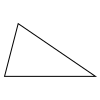
\includegraphics[width=0.6in]{output/1.models/test_watson/watson_2_true.png}\\ 
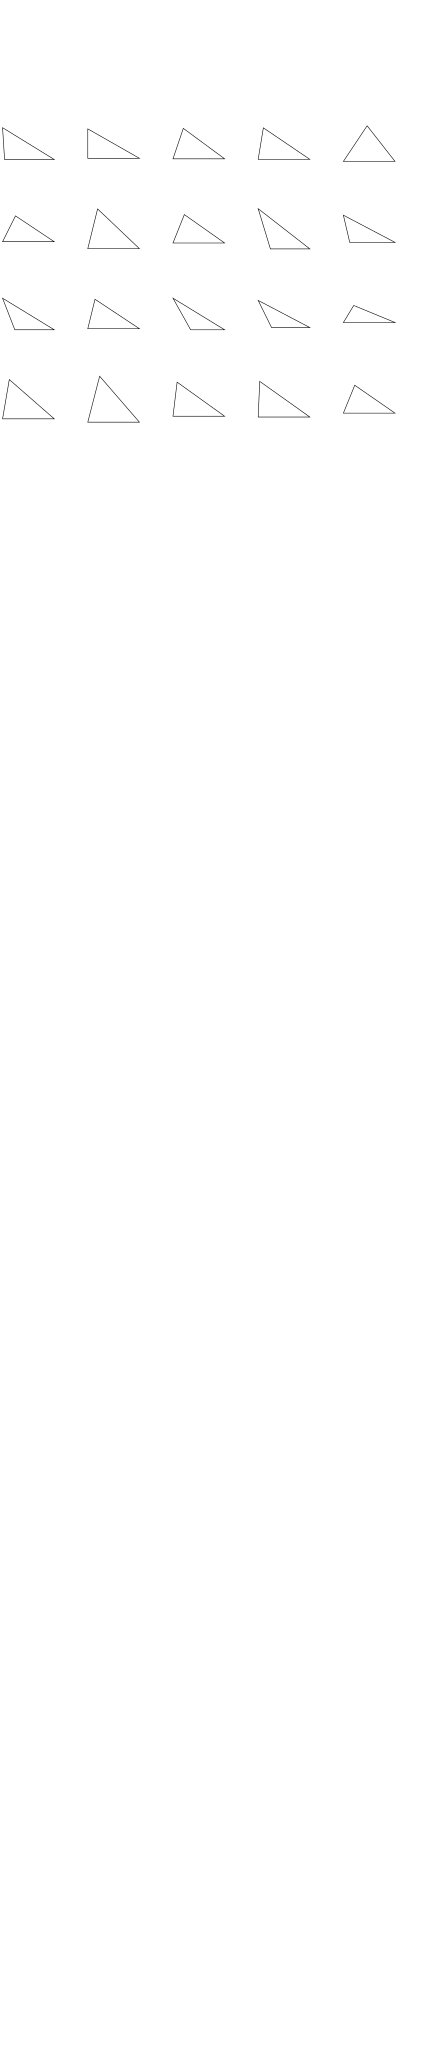
\includegraphics[width=4in]{output/1.models/test_watson/watson_2_samples.png}\\ 
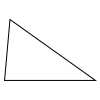
\includegraphics[width=0.6in]{output/1.models/test_watson/watson_2_est.png}
\caption{Experimenting with the Watson distribution, part 2. In the first row, the original triangle $T$. Subsequent rows are samples from Watson$(T,30.00)$. The final row is the mode of the estimated Watson distribution. The estimated concentration was $36.92$.}
\label{fig-watson-2}
\end{figure}

\begin{figure}
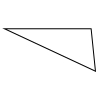
\includegraphics[width=0.6in]{output/1.models/test_watson/watson_3_true.png}\\ 
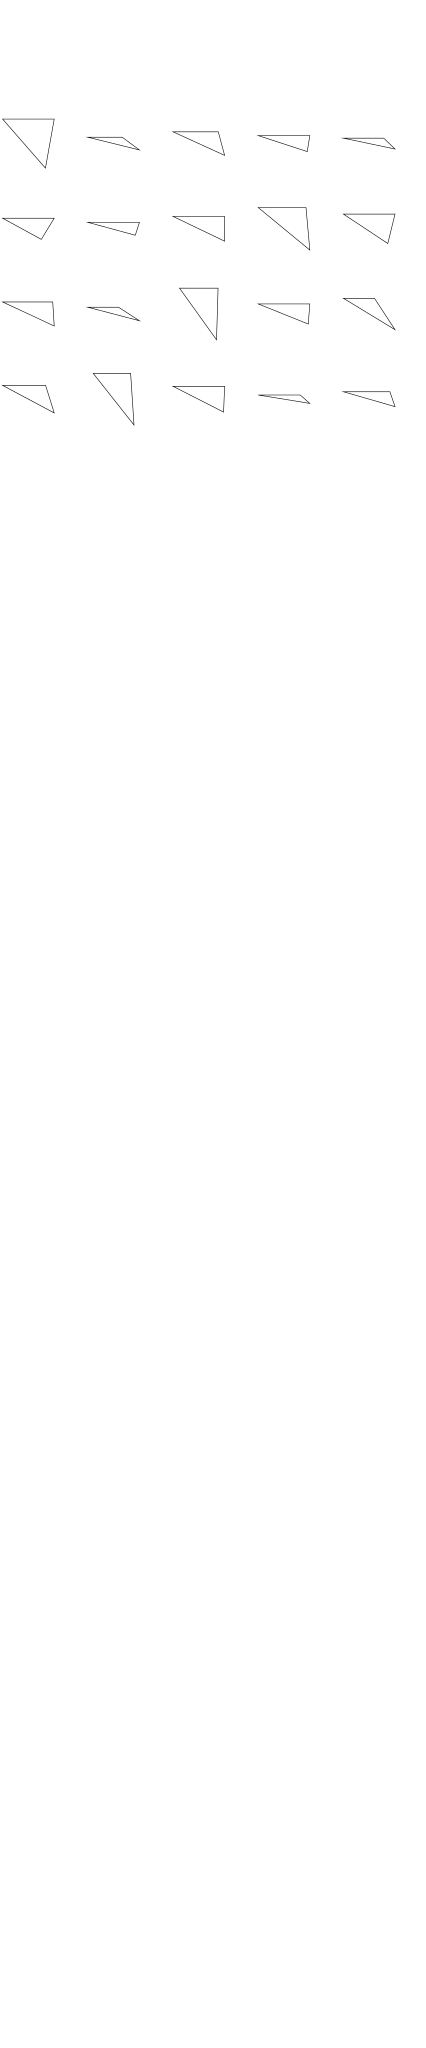
\includegraphics[width=4in]{output/1.models/test_watson/watson_3_samples.png}\\ 
\includegraphics[width=0.6in]{output/1.models/test_watson/watson_3_est.png}
\caption{Experimenting with the Watson distribution, part 3. In the first row, the original triangle $T$. Subsequent rows are samples from Watson$(T,30.00)$. The final row is the mode of the estimated Watson distribution. The estimated concentration was $21.55$.}
\label{fig-watson-3}
\end{figure}

\begin{figure}
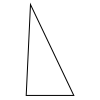
\includegraphics[width=0.6in]{output/1.models/test_watson/watson_4_true.png}\\ 
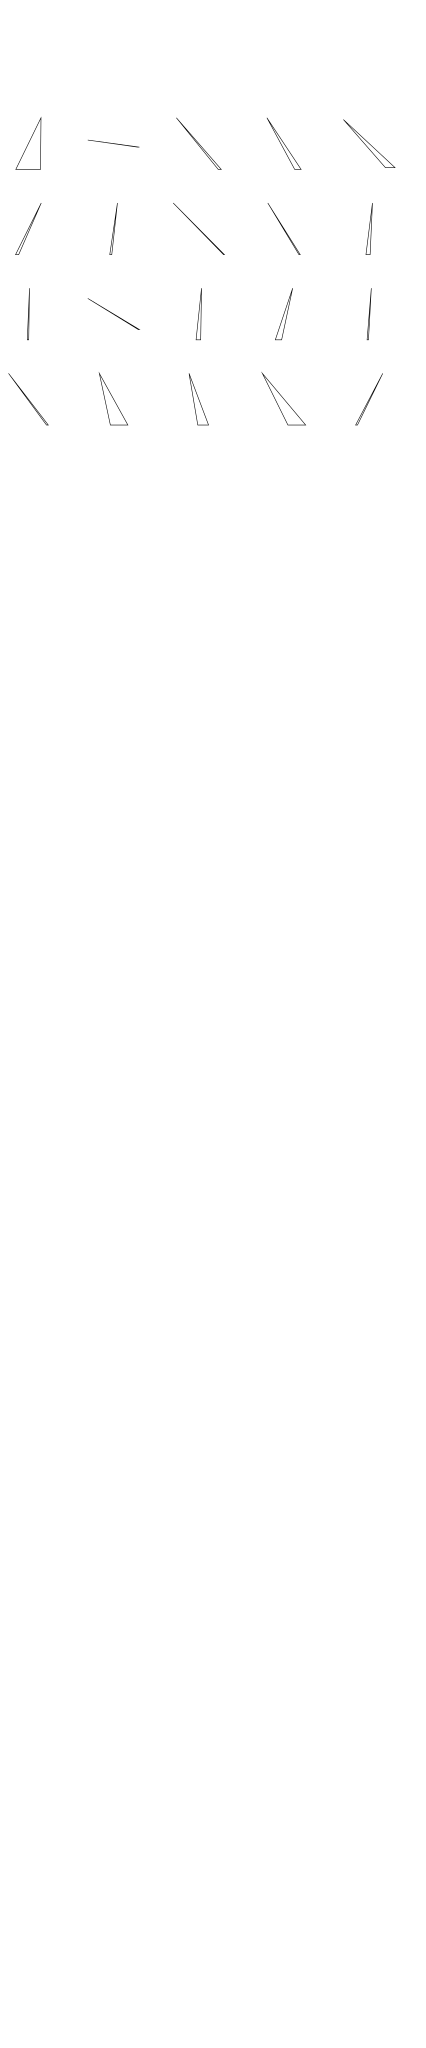
\includegraphics[width=4in]{output/1.models/test_watson/watson_4_samples.png}\\ 
\includegraphics[width=0.6in]{output/1.models/test_watson/watson_4_est.png}
\caption{Experimenting with the Watson distribution, part 4. In the first row, the original triangle $T$. Subsequent rows are samples from Watson$(T,30.00)$. The final row is the mode of the estimated Watson distribution. The estimated concentration was $92.59$.}
\label{fig-watson-4}
\end{figure}

\begin{figure}
\includegraphics[width=0.6in]{output/1.models/test_watson/watson_5_true.png}\\ 
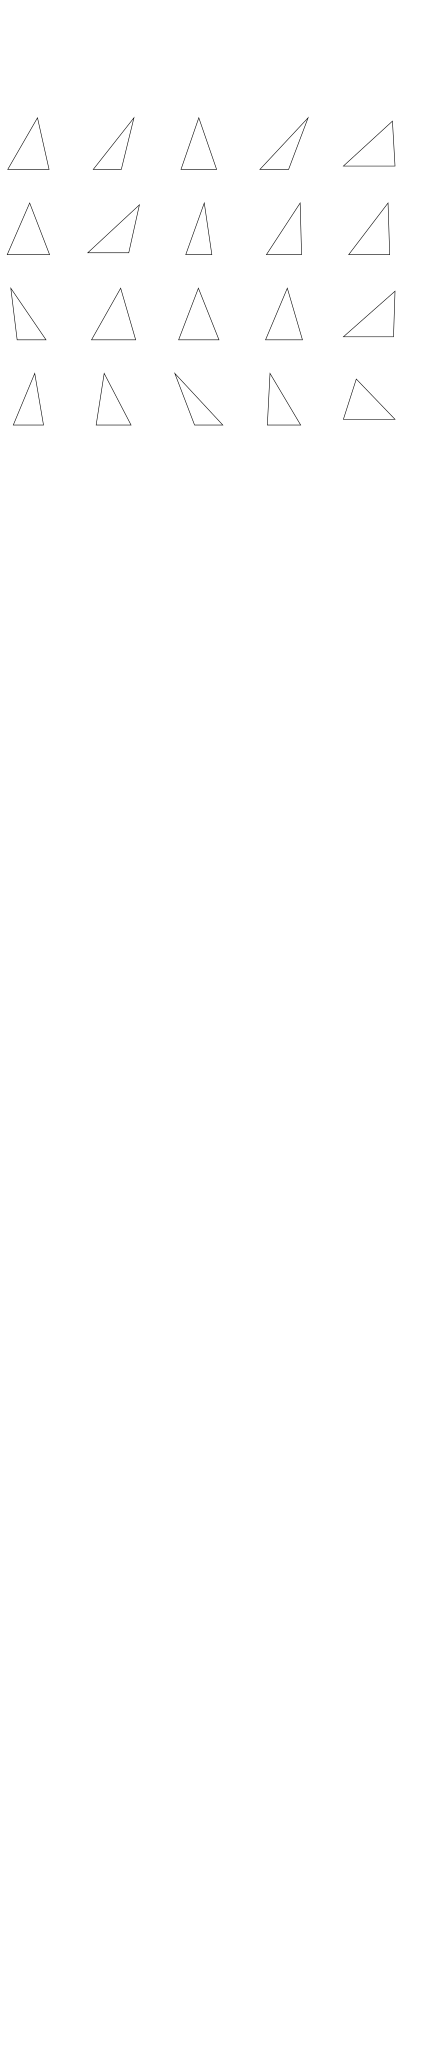
\includegraphics[width=4in]{output/1.models/test_watson/watson_5_samples.png}\\ 
\includegraphics[width=0.6in]{output/1.models/test_watson/watson_5_est.png}
\caption{Experimenting with the Watson distribution, part 5. In the first row, the original triangle $T$. Subsequent rows are samples from Watson$(T,30.00)$. The final row is the mode of the estimated Watson distribution. The estimated concentration was $31.68$.}
\label{fig-watson-5}
\end{figure}

